\documentclass{article}
%packages
\usepackage{graphicx}
\usepackage{epigraph}
\usepackage[T1]{fontenc}
\usepackage[utf8]{luainputenc}
\usepackage{amsthm}
\usepackage{amsmath}
\usepackage[font={small,it}]{caption}
%\usepackage[a5paper, total={4.5in, 7in}]{geometry} %formato libro piccolo
\usepackage[a4paper, total={7.5in, 10.35in}]{geometry} %formato libro A4
\usepackage{hyperref}
\usepackage{color,soul}
\usepackage{amsfonts}
\usepackage{amssymb}
\usepackage{imakeidx}
\usepackage{enumerate}
\usepackage{cancel}
\usepackage{physics}
\makeindex[options=-s mystyle.ist]
\usepackage{simplewick}
%\usepackage{empheq}
\usepackage{tikz}
\usepackage{graphicx}
\usepackage{braket}
\graphicspath{ {./} }
\usepackage{titlesec}
\usepackage{fancyhdr}
\usepackage{subcaption}
\usepackage{kpfonts}
\usepackage{listings}
\usepackage{xcolor}
% bibliography
\usepackage[
    backend=biber,
    style=alphabetic,
    sorting=ynt
]{biblatex}
\addbibresource{bibliography/bibliography.bib}
% algorithm
\usepackage{algorithm}
\usepackage[noend]{algpseudocode}%
% multicolumns
\usepackage{multicol}
\usepackage{lmodern}
% images folder
\graphicspath{ {./images/} }

\title{Motorize 1980 dad's telescope}

\author{Sebastiano Cocchi \& Stefano Cocchi}

\date{\today}

\begin{document}
    
    \maketitle

    \begin{abstract}
        A 1980 (old and dusty) equatorial telescope is converted to an up-to-date, motorized and computer-connected telescope.
        We, me and my father, illustrate all the transformation steps from an old, dusty and unused telescope into an optimal tool for astrophotography.
    \end{abstract}

    \tableofcontents

    % \begin{minipage}
    %     {0.6\textwidth}
    %     \tableofcontents 
    % \end{minipage}
    % \begin{minipage}
    %     {0.4\textwidth}
    %     \centering
    %     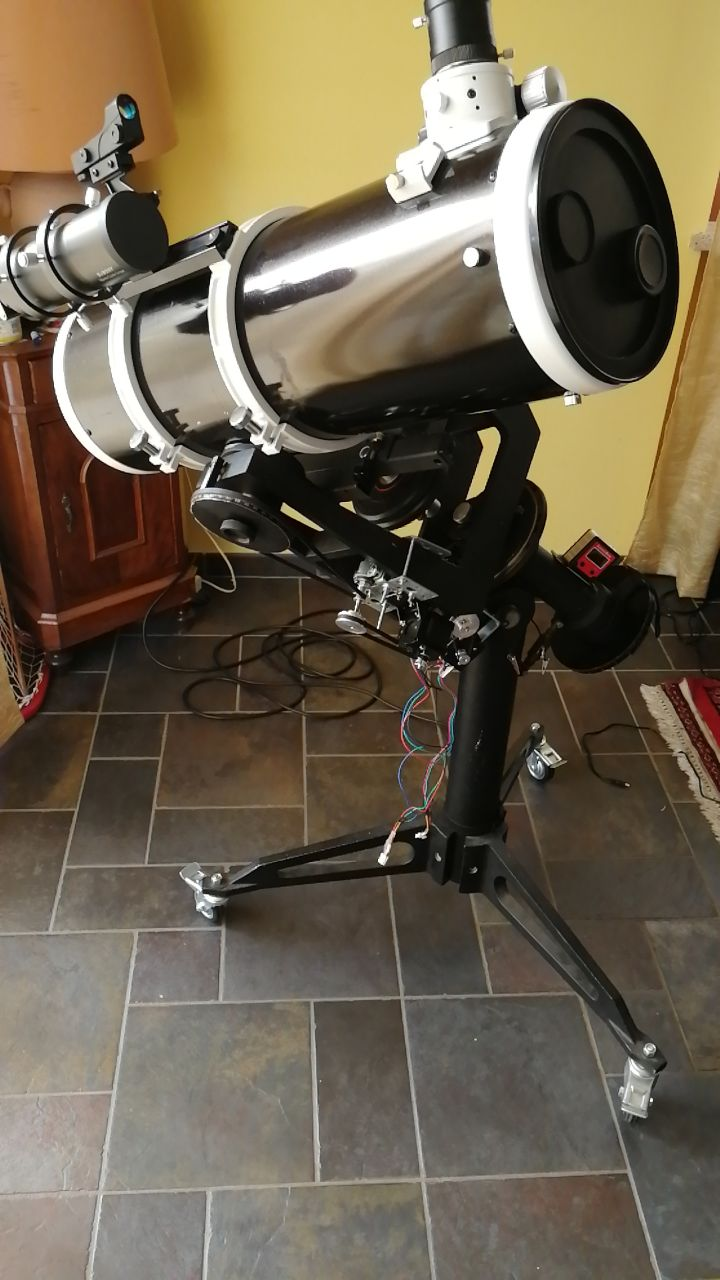
\includegraphics[scale=0.2]{telescope_image.jpg}
    % \end{minipage}

    \begin{multicols}{2}
        \section{Telescope Description}
        The starting point of the project is of course the telescope.
        In our garage, for many years, a 1980 Urania telescope has eaten a lot of dust.
        The telescope's mirror resent of years in humidity and temperature jumps in the garage.
        In the beginning, we have cleaned the silvered-mirror with soap and water, but the silver still seemed to be a bit compromised.
        We do not talk long about this telescope, since we have soon substituted it with a brand-new Skywatcher Quattro.
        The latter is placed on the Urania mount, since it is still a nice mount and, in our advice, has still not surpassed robustness.
        Indeed, the mount is a very heavy (telescope and mount totally weight 20kg!) equatorial and motorized (still works!) mount.
        
        For our money, but most importantly for our fun and entertainment, we decided to modernize our old telescope.

        \subsection{Urania telescope}
        We briefly add the specifics of the old Urania telescope, as a sort of respect for many years of honorable work before the deep dark in the garage.

        The telescope is a Urania C.R.T. NX 155, as the one in figure \ref{fig:urania_telescope_mount}.
        \\
        \begin{minipage}{0.5\textwidth}
            \centering
            \begin{tabular}{c|c}
                Specific name & value \\
                \hline
                type & reflector \\
                technique & Newton  \\
                material & PVC  \\
                weight (kg) & 10 \\
                aperture (mm) & 155 \\
                focal length (mm) & 1000 \\
                focal & f/6.5 \\
                resolution power & 0.8 \\
                limit magnitude value (mag) & 13.6 \\
                Mirror Treatment & Silica monoxide \\
                \hline
            \end{tabular}
            \captionof{table}{Urania C.R.T. NX 155 specifics.}
        \end{minipage}
        \\
        \begin{minipage}{0.5\textwidth}
            \centering
            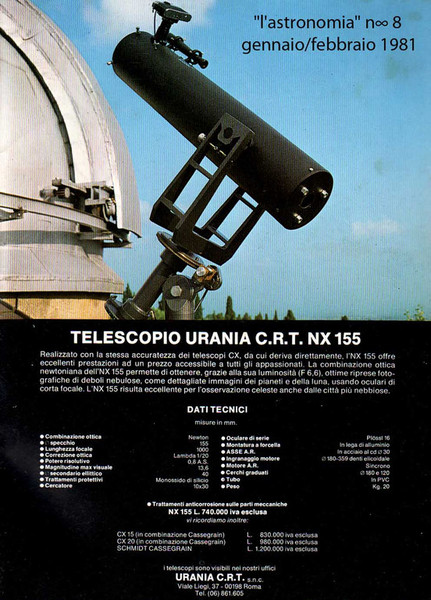
\includegraphics[scale=0.4]{urania_upper.jpg}
            \captionof{figure}{Urania telescope and mount.}
            \label{fig:urania_telescope_mount}
        \end{minipage}

        \subsection{Telescope's mount}
        The telescope is place onto an aeronautic Aluminum tripod equatorial mount.
        \\
        \begin{minipage}{.5\textwidth}
            \centering
            \begin{tabular}{cc}
                Specific & value \\
                \hline
                weight (kg) & \\
                type & fork \\
                material & Aluminum alloy \\
                RA axis diameter (mm) & 30 \\
                RA axis material & cadmium steel \\
                RA motor & 3W synchronous \\
                \hline
            \end{tabular}
            \captionof{table}{Urania's mount specifics.}
            \label{tab:mount}
        \end{minipage}

        Starting from the bottom: three pods of 30cm depart from a central post. Each one has a wheel which permits the structure to move freely and then to fix the position using stops.
        The central post terminates with the second axis holder at an inclination equal to the Earth's ecliptic \(23.43^{\circ} = 23^{\circ} 26'\).

        This axis must be aligned with the Polar star (labelling the North).
        In this way, a 3W synchronous motor can follow the sky movement.

        Departing from this second axis, a two-arms fork is free to rotate around two degrees-of-freedom defining the right ascension (RA) and the declination (DEC).
        The two arms are separated by the distance \(d = 15\)mm which is the Urania telescope aperture.
        \subsection{Skywatcher 8P Quattro telescope}
        Skywatcher 8P Quattro Newtonian telescope (figure \ref{fig:skywatcher_telescope_mount}) offers an optimal astrophotography performance.
        For this reason we have decided to substitute the Urania telescope with this brand-new Skywatcher telescope.
        \\
        \begin{minipage}{0.5\textwidth}
            \centering
            \begin{tabular}{c|c}
                Specific name & value \\
                \hline
                type & reflector \\
                technique & Newton  \\
                material & Carbon  \\
                weight (kg) & 8.0 \\
                aperture (mm) & 200 \\
                focal length (mm) & 800 \\
                focal & f/4 \\
                resolution power & 0.58 \\
                limit magnitude (mag) & 13.3 \\
                collect light & 820 \\
                magnification & 400 \\
                Mirror Treatment & Aluminum Coating \\
                Focuser & Crayford dual-speed 50.8/31.8 \\
                \hline
            \end{tabular}
            \captionof{table}{Skywatcher 8P Quattro}
            \label{tab_skywatcher_quattro}
        \end{minipage}
        \\
        \begin{minipage}{0.5\textwidth}
            \centering
            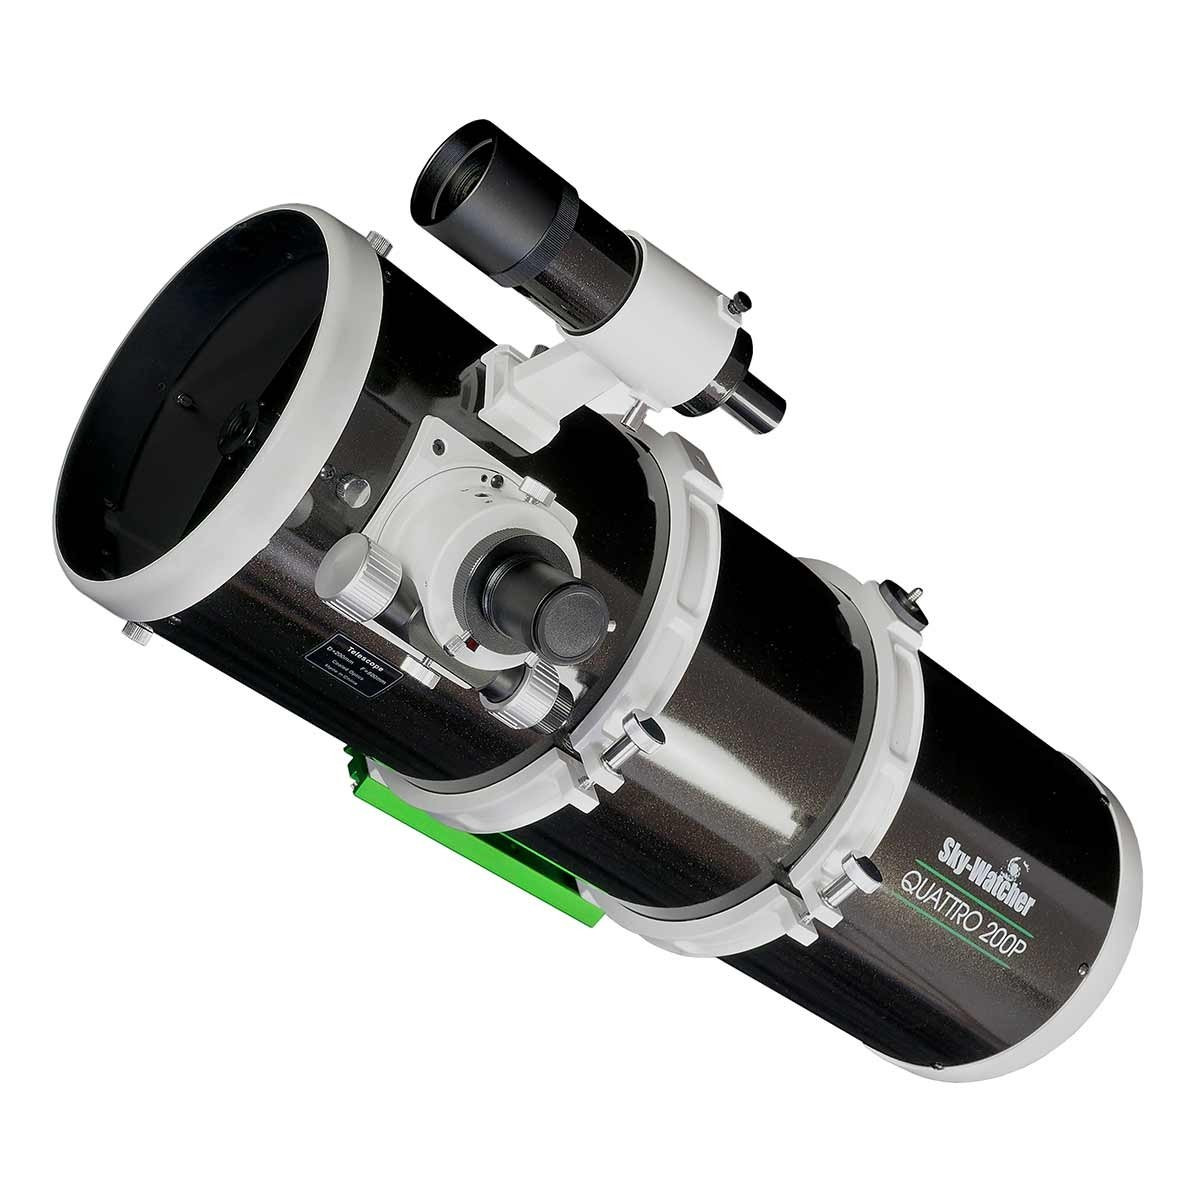
\includegraphics[scale=0.2]{newton-quattro-200-sky-watcher.jpg}
            \captionof{figure}{Skywatcher Quattro telescope.}
            \label{fig:skywatcher_telescope_mount}
        \end{minipage}
        \\
        Since the Skywatcher telescope does not fit in the fork, we have thought to build a "saddle" onto which placing the telescope.
        The specifics of this installation are shown in the following section.
         

        \section{Telescope substitution: from Urania's tube to Skywatcher's tube}
        Passing from the Urania telescope to Skywatcher telescope we have faced the problem of how to insert the latter in the telescope mount.
        Indeed, since Skywatcher's telescope diameter is 200mm it does not fit inside the mount fork.

        Our solution is to insert a seat in which to place the telescope.
        The barycenter of the telescope is not centered with the DEC axis, thus we have settled a post capable of holding weights to balance the forces.
        See figure \ref{fig:piastra_DEC} and \ref{fig:piastra_particular}.
        \\
        \begin{minipage}{0.25\textwidth}
            \centering
            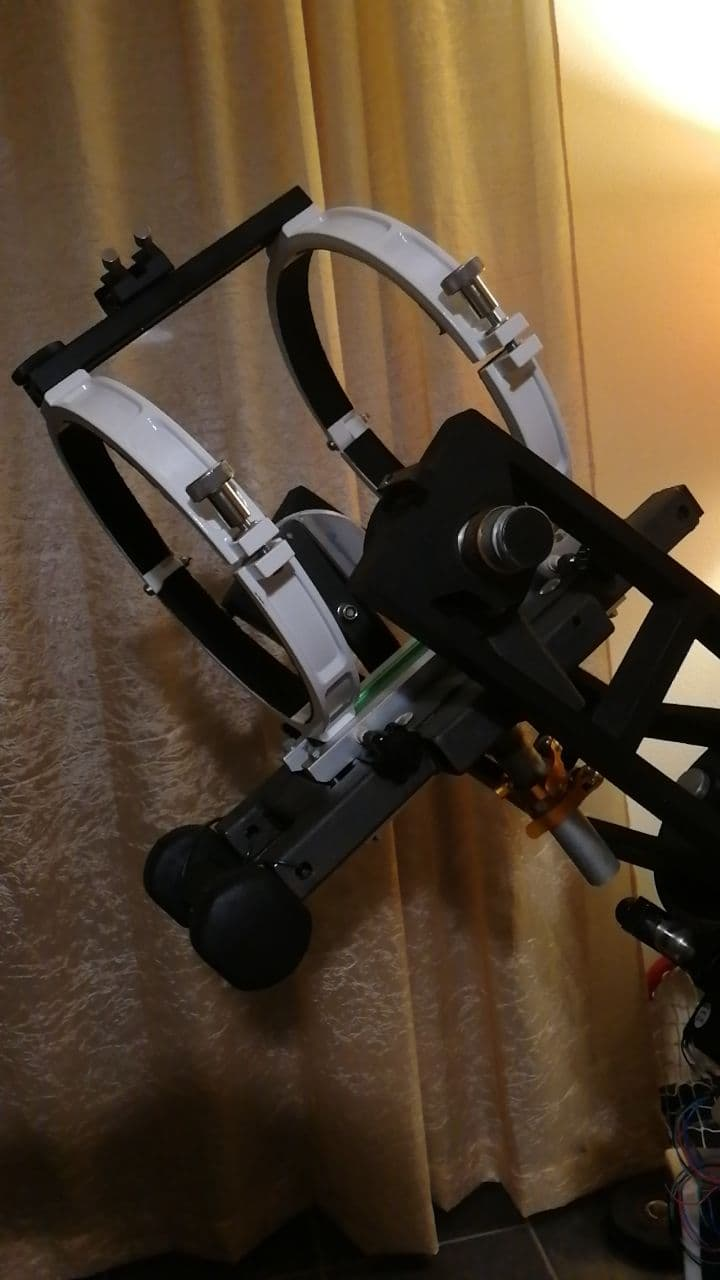
\includegraphics[scale=0.5]{DEC_sede.jpg}
            \captionof{figure}{The mechanism built to insert Skywatcher's telescope into the Urania robust mount.}
            \label{fig:piastra_DEC}
        \end{minipage}
        \begin{minipage}
            {0.25\textwidth}
            \centering
            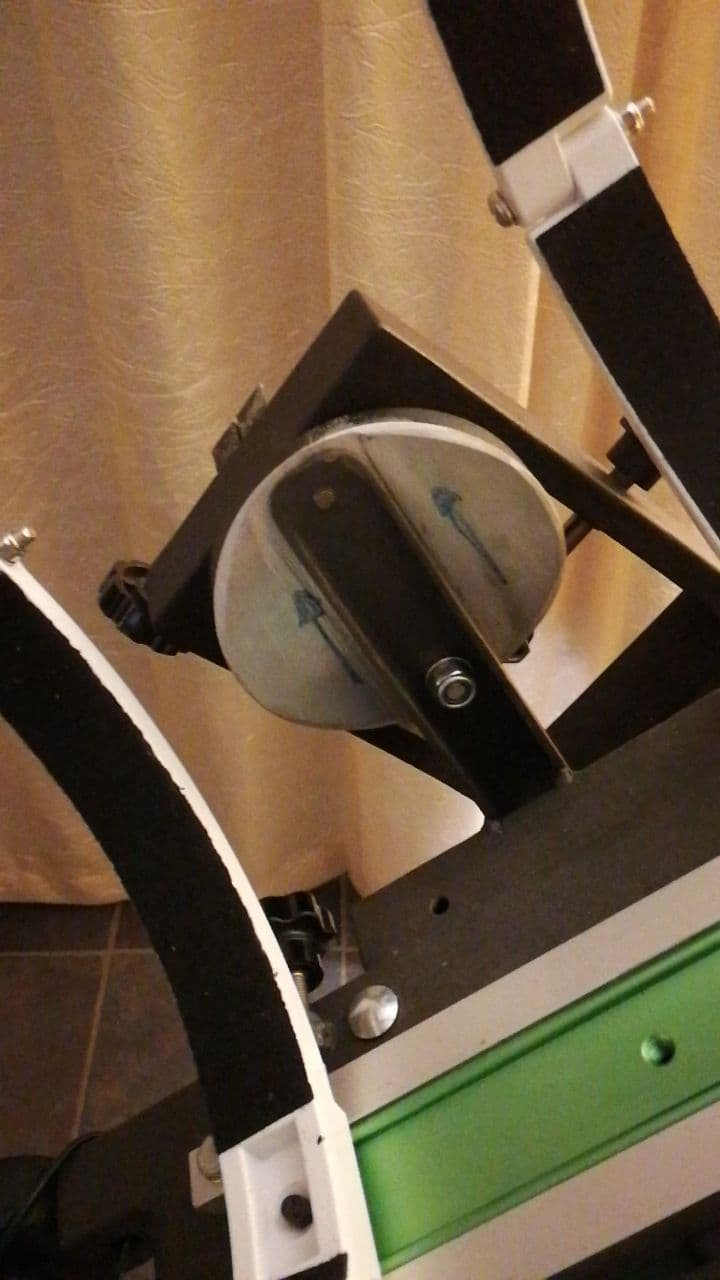
\includegraphics[scale=0.5]{DEC_piastra.jpg}
            \captionof{figure}{detail of the replacement plate that supports the new telescope.}
            \label{fig:piastra_particular}
        \end{minipage}
        \\
        The scheme with distances is visible in figure \ref{fig:DEC_piastra_dimensioni}.
        \\
        \begin{minipage}
            {0.5\textwidth}
            \centering
            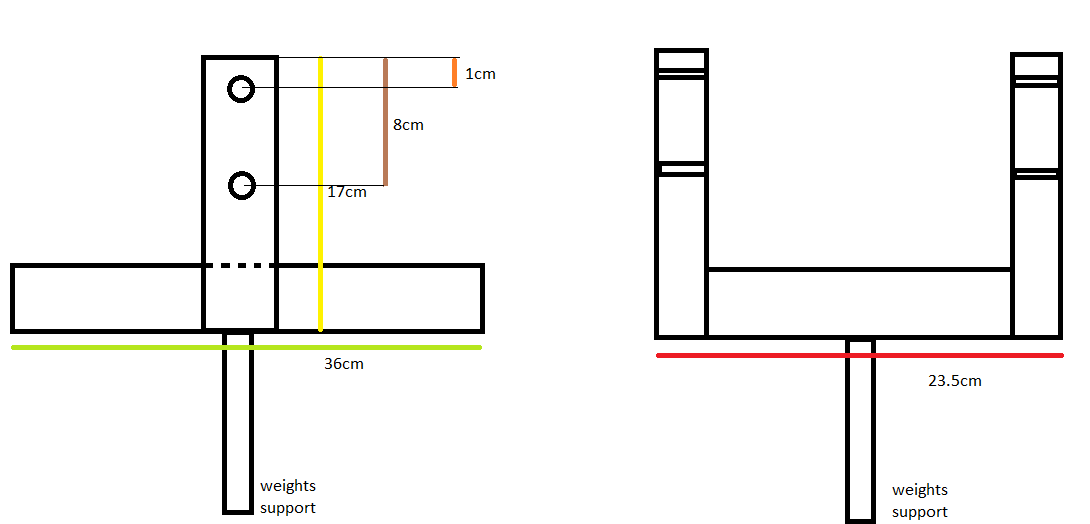
\includegraphics[scale=0.75]{DEC_piastra_dimensioni.png}
            \captionof{figure}{Schematic view of the telescope mount insertion.
            This represents only the installation build with some squared metal bars upon which the two white loops (which hold the telescope tube) are fixed and are not illustrated in this scheme. The two holes in each arm serve to fix the structure on the mount. }
            \label{fig:DEC_piastra_dimensioni}
        \end{minipage}

        \section{Motorization: microcontrollers}
        \subsection{The Arduino experience}
        We decide to write this section more as an advertisement to not follow this way than for other purposes.

        The first, natural, approach was to try to use some at-home-technology.
        Alone on a shelf, an Arduino UNO R3 card was waiting to take part of another project with some friends: a 28BYJ-48 stepper motor and colorful cables.
        What a better occasion to be mounted on the telescope in turns of the 3W motor?

        With some fortunate events, the stepper motor is adapted to the telescope's RA rotating worm shaft.
        Was it good as a tracker motor with a constant motion?
        The answer is no.
        Indeed, some tests revealed bad performances like the inconstant rotation and several stops due to lack of robustness of the motor.
        This result was easily supposed from the beginning, but this try was costs-less, \(i.e.\) free since all the components were at home.
        Indeed, citing Wayne Gretzky:
        \begin{quote}
            "you miss one hundred percent of the shots you don't take",
        \end{quote}
        so it was a matter of must-a-do proof.
        It also gave us the opportunity to face some \textit{engineering} problems.
        
        During a little internet journey, we have found a new stepper motor with a nema 17 standard;
        we have bought two kinds: one of the more robust stepper motors on store and one less robust.
        
        The 28BYJ-48 stepper motor, sadly, returns onto its shelf as, shortly after, would do the Arduino UNO card.

        \subsection{Stepper motors}
        In this subsection we write the specifics of the stepper motors used for the RA and DEC mechanization (for both we have used nema 17 motors) and the focuser (developed with a nema 11 stepper motor).

        \subsubsection{RA stepper motor}
        \begin{minipage}{0.5\textwidth}
            \centering
            \begin{tabular}{cc}
                \textbf{17HM15-0904S stepper motor}&\\
                Electronics&\\
                \hline
                Manufacturer code & 17HM15-0904S\\
                Engine type & bipolar\\
                Pitch angle (deg) & 0.9 \\
                Torque (Ncm)& 36\\
                Rated current/phase (A) & 0.9\\
                Phase resistance (Ohm)& 60\\
                Voltage (V)& 5.4\\
                Inductance (mH)& 12 \(\pm\) 20\% (1 kHz)\\
                 & \\
                Physical specifications&\\
                \hline
                Frame dimensions (mm\(^2\))& 42x42 \\
                Body length (mm)& 40 \\
                Shaft diameter (mm)& 5 \\
                Stem length (mm)& 22 \\
                D-cut length (mm)& 15 \\
                Number of cables & 4\\
                Lead number (mm)& 300 \\
                Weight (g) & 280\\
                \hline
            \end{tabular}
            \captionof{table}{Nema 17 stepper motor for the RA motion specifics.}
            \label{tab:nema_17_specifics}
        \end{minipage}

        \subsubsection{DEC stepper motor}
        
        \begin{minipage}{0.5\textwidth}
            \centering
            \begin{tabular}{cc}
                \textbf{17HM19-2004S1 stepper motor}&\\
                Electronics&\\
                \hline
                Manufacturer code & 17HM19-2004S1\\
                Engine type & bipolar\\
                Pitch angle (deg) & 0.9 \\
                Torque (Ncm)& 46\\
                Rated current (A) & 2\\
                Phase resistance (Ohm)& 1.4\\
                Voltage (V)& 2.8\\
                Inductance (mH)& 4\\
                 & \\
                Physical specifications&\\
                \hline
                Frame dimensions (mm\(^2\))& 42x42 \\
                Body length (mm)& 48 \\
                Shaft diameter (mm)& 5 \\
                Stem length (mm)& 24 \\
                D-cut length (mm)& 24 \\
                Number of cables & 4\\
                Lead number (mm)& 500 \\
                Weight (g) & 370\\
                \hline
            \end{tabular}
            \captionof{table}{Nema 17 stepper motor for the DEC motion specifics.}
            \label{tab:nema_17_specifics_2}
        \end{minipage}

        \subsubsection{Focuser stepper motor}
        \begin{minipage}{0.5\textwidth}
            \centering
            \begin{tabular}{cc}
                \textbf{11HS12-0674S stepper motor}&\\
                Electronics&\\
                \hline
                Manufacturer code & 11HS12-0674S\\
                Engine type & bipolar\\
                Pitch angle (deg) & 1.8 \\
                Torque (Ncm)& 7\\
                Rated current (A) & 0.67\\
                Phase resistance (Ohm)& 5.6\\
                Voltage (V)& 3.8\\
                Inductance (mH)& 4.2\\
                 & \\
                Physical specifications&\\
                \hline
                Frame dimensions (mm\(^2\))& 28x28 \\
                Body length (mm)& 31.5 \\
                Shaft diameter (mm)& 5 \\
                Stem length (mm)& 20 \\
                Number of cables & 4\\
                Lead number (mm)& 300 \\
                Weight (g) & 110\\
                \hline
            \end{tabular}
            \captionof{table}{Nema 11 stepper motor for the focuser motion specifics.}
            \label{tab:nema_11_specifics}
        \end{minipage}

        \subsection{ESP32}
        After buying the new stepper motor, on the internet we have found good impressions on the ESP32 microcontroller.
        ESP32 is a series of low-cost, low-power system on a chip microcontroller with integrated Wi-Fi and dual-mode Bluetooth.
        We've bought the ESP32 D1 R32, the one in figure \ref{fig:esp32}, for better attaching the motor using the CNC shield V3 (which is briefly explained in the following).
        Also, Arduino returned on the self with its friends.

        We bumped into a OnStep project (at \url{https://onstep.groups.io/g/main/wiki/19670}) which an open source software providing the control of four stepper motors (RA, DEC, focuser and rotator for astrophotography), weather sensor handling, Wi-Fi and Bluetooth connection, polar alignment and other nice features.
        We decided to follow the "Wemos R32 and CNC V3" project.
        
        \begin{minipage}
            {.5\textwidth}
            \centering
            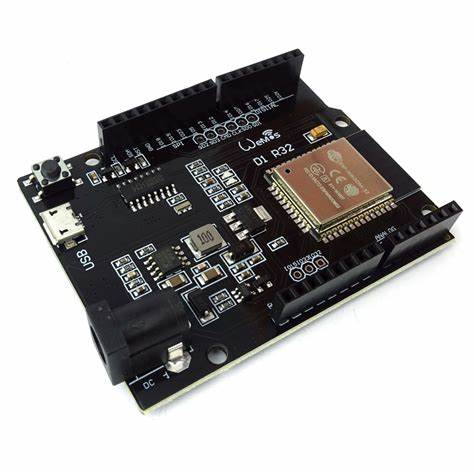
\includegraphics[scale=0.28]{esp32_d1_r32.jpg}
            \captionof{figure}{ESP32 D1 R32 picture.}
            \label{fig:esp32}
        \end{minipage}

        \subsection{CNC Shield V3}
        To better optimize space and wires connections, we have bought a CNC Shield V3 (\(aka\) CNC3), see figure \ref{fig:cnc3}.
        \begin{minipage}
            {0.5\textwidth}
            \centering
            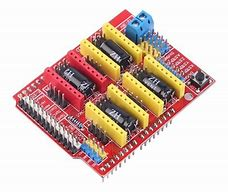
\includegraphics[scale=0.5]{CNC3.jpg}
            \captionof{figure}{CNC3 Shield V3.}
            \label{fig:cnc3}
        \end{minipage}
        It is an add-on shield, built to be used for 3D printers.
        It has 4 slots, each one can host a motor driver.

        \subsection{Motor drivers}
        On the CNC3 shield, we have put two DRV8828 drivers and adjusted the currents using a screwdriver and a multimeter to the values in table \ref{tab:drivers_curr}

        \begin{minipage}
            {.5\textwidth}
            \centering
            \begin{tabular}{cc}
                Motor & Current (A) \\
                \hline
                RA motor & 0.45 \\
                DEC motor & 0.9 \\                
            \end{tabular}
            \captionof{table}{DRV8828 drivers setup current.}
            \label{tab:drivers_curr}
        \end{minipage}

        \subsection{Power supply}
        The power supply is provided by a 19V 5A power supply as in table \ref{tab:power_supply}.

        \begin{minipage}
            {.5\textwidth}
            \centering
            \begin{tabular}{cc}
                 voltage output (V) & current output (A) \\
                 \hline
                19.3 & 4.74 \\
            \end{tabular}
            \captionof{table}{Nominal tension and current outputs of the power supply.}
            \label{tab:power_supply}
        \end{minipage}

        For our initial purposes it was enough, indeed 5A are enough to feed quite well two stepper motors and a poor electronics.
        A rough estimation poses 1.8A for DEC motor, 0.9A for RA motor and few milliampéres for the ESP32. 
        The reader is strongly encouraged to check the total current its circuit needs before buying a power supply.

        \subsection{Sensors: Wi-Fi connection, Real time clock (RTC) and weather sensor (BMP280)}
        An ESP8688 WeMos D1 mini is connected to the CNC3 as shown in \url{https://onstep.groups.io/g/main/wiki/19670}.

        This OnStep has a software addon called the Smart Web Server (SWS) which provides WiFi or Ethernet connections over IP.
        Many devices support this type of connection including cell-phones, tablets, laptop/desktop computers, etc.
        Using this library, it is possible to use programs such as Stellarium via ASCOM drivers provided by the OnStep project \url{http://www.stellarjourney.com/index.php?r=site/software_telescope}.

        \section{Motorization: the mechanics}
        The motorization of the telescope passes through two mechanics adjustments:
        \begin{enumerate}
            \item motorize the RA movement, exploiting the native tracker mechanism;
            \item motorize the DEC movement, which natively has no gears.
        \end{enumerate}

        \subsection{RA motorization}
        The telescope's mount has already a tracking mechanism motorized by a 3W synchronous motor.
        So, in principle, it is only a matter of substitute this old motor, with a new programmable stepper motor.

        The gears are composed by:
        \begin{itemize}
            \item a 359 teeth stage (1 tooth for each degree, fantastic);
            \item an endless screw (worm) mounted on a shaft through a clutch.
        \end{itemize}
        Using this structure, for a continuous sky tracking, the elder motor would complete a round of the worm in 4 minutes.
        Thus, this mechanism rotates the mount with the velocity of a degree in 4 minutes (which is the velocity of the sky moving away in the night).

        We have reduced the ratio by a third adding two other gears (see figure \ref{fig:RA_mechanization}): 60 teeth gear positioned in the shaft and a 20 teeth gear on the motor shaft.
        \\
        \begin{minipage}{.5\textwidth}
            \centering
            \begin{tabular}{cc|c}
                ratio gear 1 & ratio gear 2 & total ratio \\
                \hline
                1/360 & 1/3 & 1/1080 \\
                \hline
            \end{tabular}
            \captionof{table}{Total reduction of RA mechanization.}
            \label{tab:RA_mechanization}
        \end{minipage}
        \\
        \begin{minipage}{.5\textwidth}
            \centering
            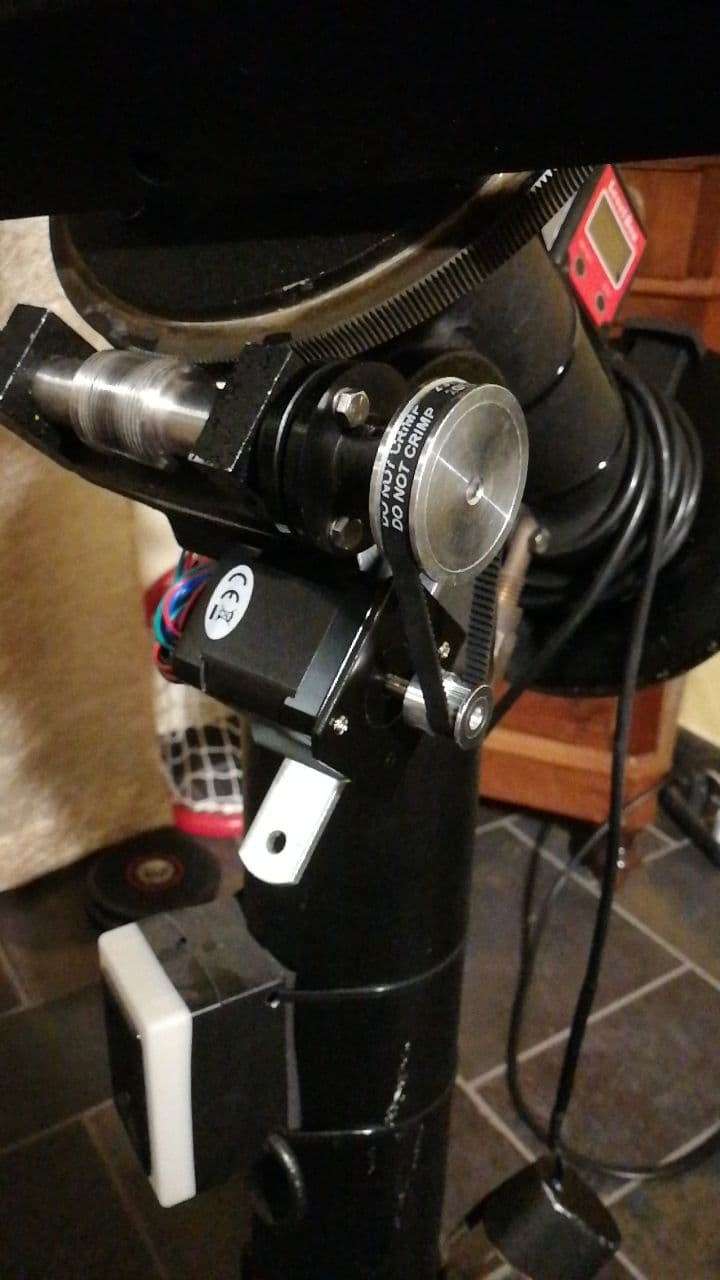
\includegraphics[scale=0.6]{RA_motorization.jpg}  
            \captionof{figure}{Nema 17 stepper motor and gear adjustment.}
            \label{fig:RA_mechanization}         
        \end{minipage}
        \\
        We have choose to install a nema 17 stepper motor with the specifics in table \ref{tab:nema_17_specifics}

        \subsection{DEC motorization}
        The mechanization of the DEC axis was a bit more complicated since there was not a built-in gear to use.
        We tried different versions.
        A first successfully try was to exploit a stand-alone disk.
        On the edge of the latter are present some ticks and grades: it was used a declination angle teller.

        As told above, we have tried different configurations but same stepper motor is used.

        \subsubsection{DEC V1}
        The first version is made using the built-in graded disk mounted on the telescope.
        On this, is attached a 32cm long chain strip.
        Then, a 1/3 reduction shaft is positioned between the first gear and the stepper motor's gear.
        The total reduction with all gear specifics is reported in table \ref{tab:DEC_gear_spec}.
        Figure \ref{fig:DEC_mechanism} is a picture of the mechanism.

        \begin{minipage}
            {0.5\textwidth}
            \centering
            \textbf{DEC-V1 stages}\\
            \begin{tabular}{ccccc}
                \hline
                Gear number & 1 & 2 & 3 & 4 \\
                number of teeth & 188 & 20 & 60 & 20 \\
                \hline
                total ratio & \(\sim \frac{1}{28}\) &&&
            \end{tabular}
            \captionof{table}{DEC mechanism's gear specifics.}
            \label{tab:DEC_gear_spec}
        \end{minipage}
        \\
        \begin{minipage}
            {0.5\textwidth}
            \centering
            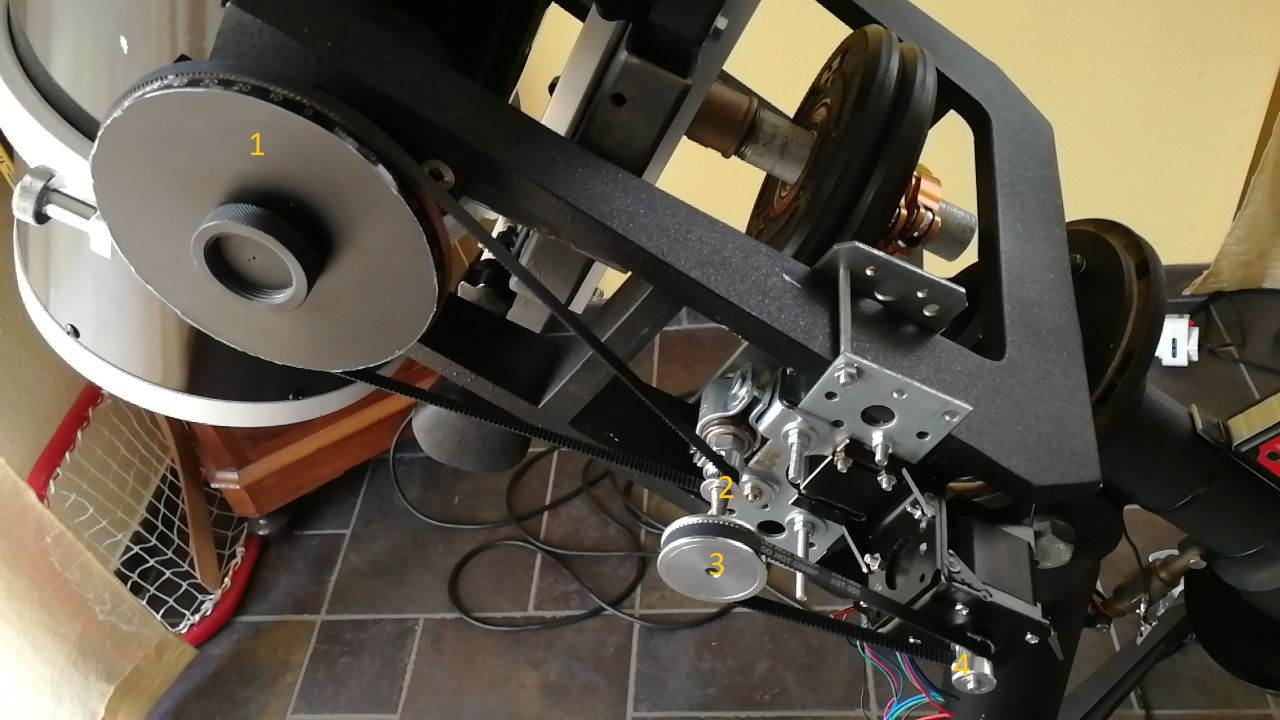
\includegraphics[scale=.28]{DEC_motorization.jpg}
            \captionof{figure}{DEC mechanism.}
            \label{fig:DEC_mechanism}
        \end{minipage}
        \\
        This solution seemed to be efficient, but easy to adjust.
        Also, the stage reduction is too low for a good movement precision.

        \subsubsection{DEC V2}
        The second version is made uses again the built-in graded disk mounted on the telescope.
        Also on this construction is glued a 32cm long chain strip.
        Then, a 1/9 reduction is positioned between the first stage and the stepper motor.
        The total reduction with all gear specifics is reported in table \ref{tab:DEC_gear_spec_v2}.
        Figure \ref{fig:DEC_mechanism_v2} is a picture of the mechanism.

        \begin{minipage}
            {0.5\textwidth}
            \centering
            \textbf{DEC-V2 stages}\\
            \begin{tabular}{ccccccc}
                \hline
                Gear number & 1 & 2 & 3 & 4 & 5 & 6\\
                number of teeth & 188 & 20 & 60 & 20 & 60 & 20\\
                \hline
                total ratio & \(\sim \frac{1}{84}\) &&&
            \end{tabular}
            \captionof{table}{DEC mechanism's gear specifics.}
            \label{tab:DEC_gear_spec_v2}
        \end{minipage}
        \\
        \begin{minipage}
            {0.5\textwidth}
            \centering
            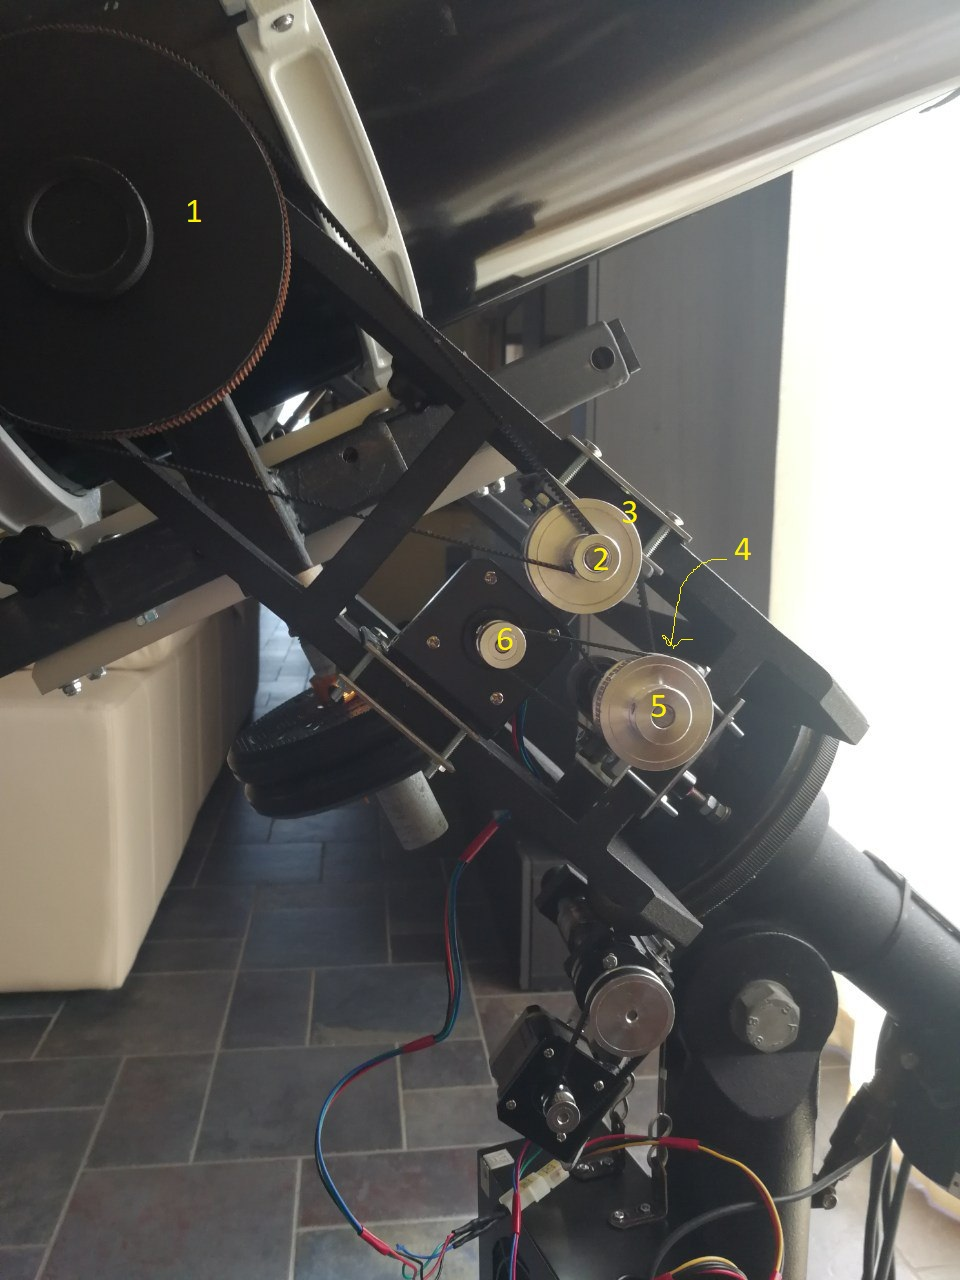
\includegraphics[scale=.2]{DEC_v2.jpg}
            \captionof{figure}{DEC V2 mechanism.}
            \label{fig:DEC_mechanism_v2}
        \end{minipage}
    
        \subsection{Focuser motorization}
        Another improvement is the motorization of the focuser.
        Using a nema 11 stepper motor, we have created the motor supports and the gears using a 3D printer.
        The reduction stage is 3.


        \section{Cable management}
        The wiring between the electronics and the motors is made focusing on the main idea to attach and detach them rapidly.
        We thought to use Ethernet cables.
        They are a versatile solution but how to connect them to the four cables governing the stepper motor?

        Stepper motors have four cables, see figure \ref{fig:stepper-motors-cables}, which have to be driven to the CNC3.
        \\
        \begin{minipage}
            {0.5\textwidth}
            \centering
            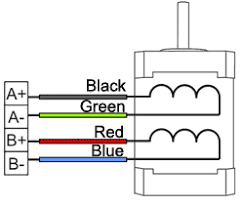
\includegraphics[scale=0.5]{stepper-motors-cables.png}
            \captionof{figure}{Stepper motor cables scheme.}
            \label{fig:stepper-motors-cables}
        \end{minipage}

        \subsection{Ethernet cables}
        Ethernet cables are composed typically by 8 thin cables, each one carrying very few Amperes, approximately \(0.3-0.5A\).
        Since stepper motors require currents of the order of \(1A\), we decided to use them in couple, according to the general Ethernet cabling scheme.
        Thus, the four motor cables are doubled and fixed into the eight way Ethernet socket.

        Then, the main box is prepared to receive the Ethernet cables.
        In the most remote drawers of the garage, we have found an old and burned electronic card with four Ethernet sockets, a power supply entry and an on/off switch.
        Using a multimeter we have checked the pins of each slot and created the connections to the CNC3 shield.

        In figures \ref{fig:box}, \ref{fig:RA-box} and \ref{fig:fouser-box} are shown some examples of Ethernet wiring.

        \subsection{Plastic boxes}
        Using a 3D printer, we have created the focuser motor box with the Ethernet exit, and so we did for the RA motor.
        The microcontroller, the CNC3 shield, the power supply and all the electronics have been thrown in a box.
        The stepper motors drivers after a while become very hot, then we have decided to put a fan in the box.
        In figures \ref{fig:box}, \ref{fig:RA-box} and \ref{fig:fouser-box} are shown the resulting plastic boxes.

        \begin{minipage}
            {0.5\textwidth}
            \centering
            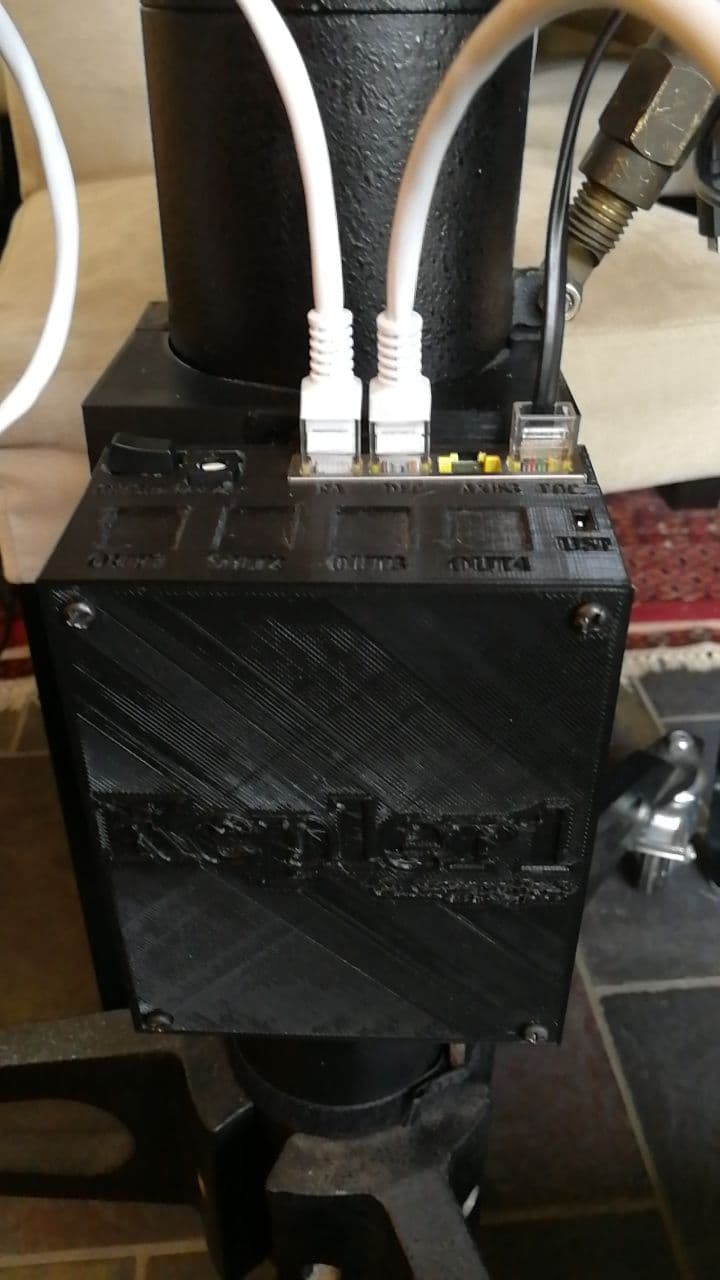
\includegraphics[scale=0.5]{BOX.jpg}
            \captionof{figure}{The main box containing the electronics and its easy management Ethernet connections.}
            \label{fig:box}
        \end{minipage}

        \begin{minipage}
            {0.5\textwidth}
            \centering
            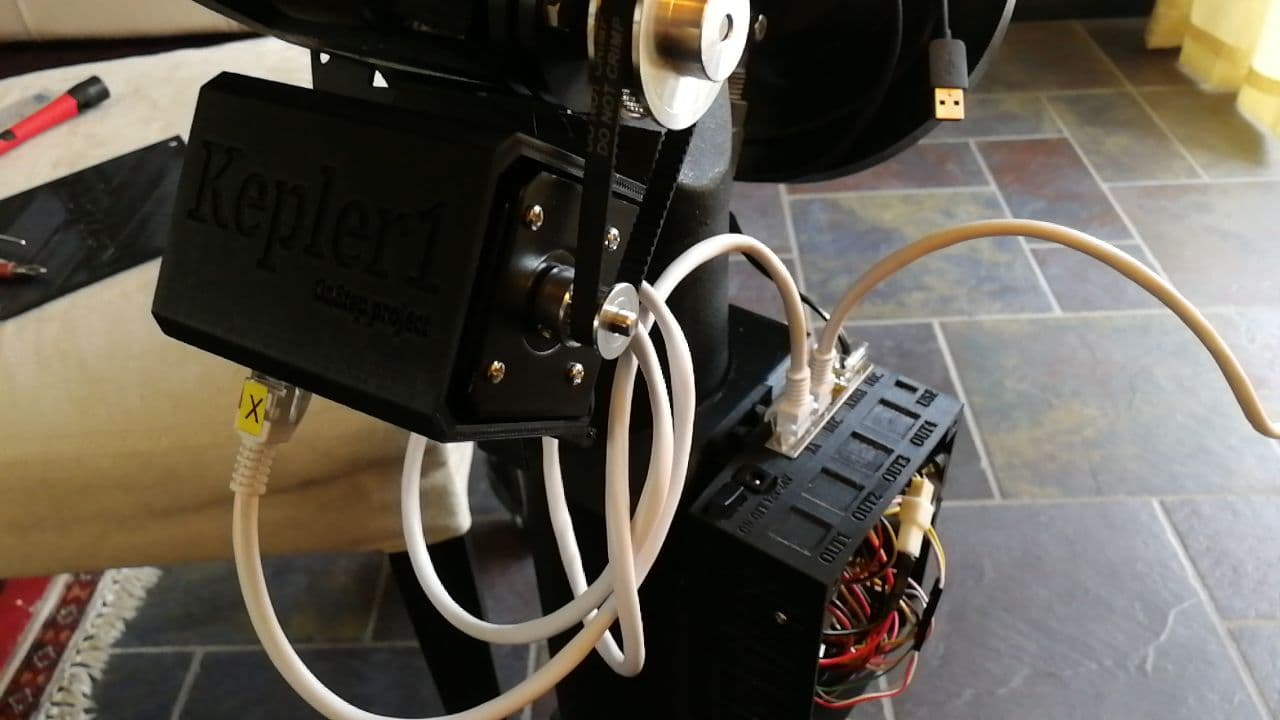
\includegraphics[scale=0.5]{RA-box.jpg}
            \captionof{figure}{The RA motor box containing the stepper motor and its Ethernet socket.}
            \label{fig:RA-box}
        \end{minipage}

        \begin{minipage}
            {0.5\textwidth}
            \centering
            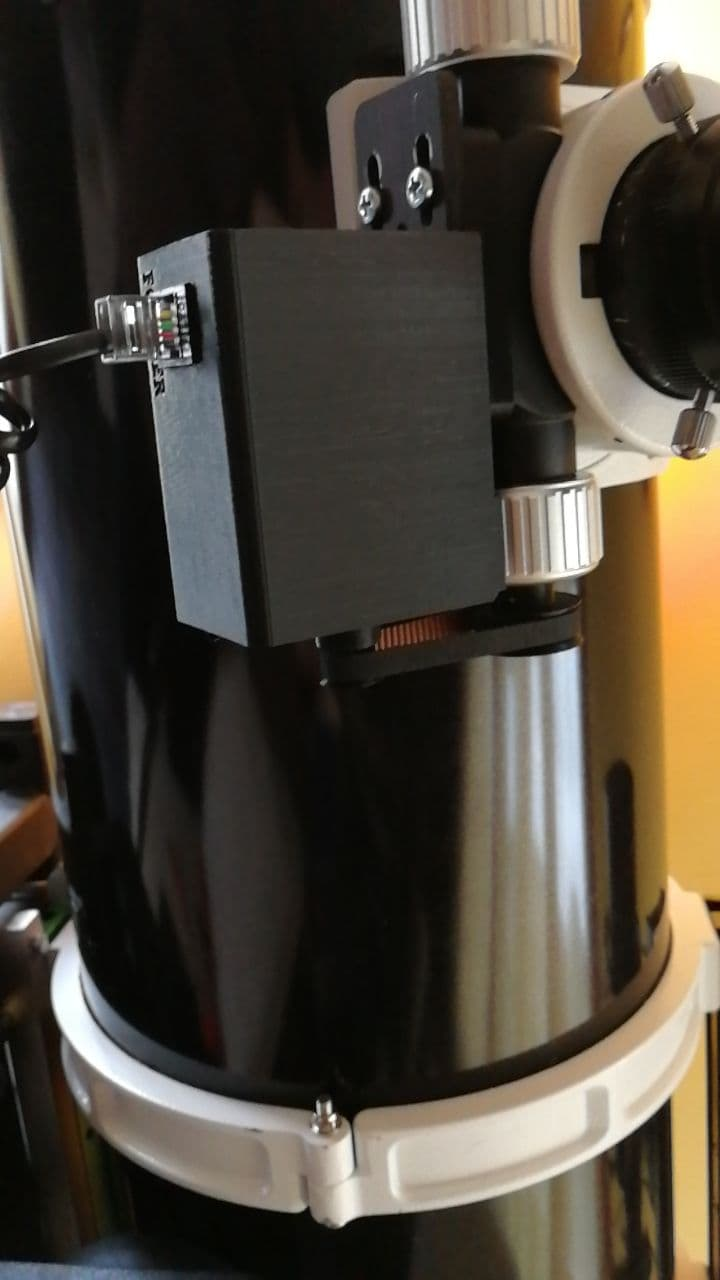
\includegraphics[scale=0.5]{FOCUSER-box.jpg}
            \captionof{figure}{The focuser box containing the focuser stepper motor and its Ethernet socket.}
            \label{fig:focuser-box}
        \end{minipage}

        \section{The software}
        Now comes the software part.
        In our mind, we wouldn't want to spend much time on programming.
        We desired a plug-and-play solution, or something similar.
        A software with easily controlling and possibly which can talk via ASCOM drivers with Stellarium (or others), PHD2 and others astrophotography programs.

        \subsection{OnStep}
        On the internet, we have found a great, open-source, free and customizable software called OnStep.\footnote{Wiki groups:\url{https://onstep.groups.io/g/main/wiki/3860}.\\Github:\url{https://github.com/hjd1964/OnStep}.}
        We have followed the instructions for the WeMos D1 \(+\) CNC V3 project, configured the Config.h file and upload the sketch on the ESP32 board.
        \begin{minipage}
            {0.5\textwidth}
            \centering
            \begin{tabular}{cc}
                Variable & value \\
                \hline
                \texttt{PINMAP} & CNC3\\
                \texttt{SERIAL\_A\_BAUD\_DEFAULT} & 115200 \\
                \texttt{SERIAL\_B\_BAUD\_DEFAULT} & 115200 \\
                \texttt{SERIAL\_C\_BAUD\_DEFAULT} &  ON \\
                \texttt{MOUNT\_TYPE} & FORK \\
                \texttt{BUZZER} & ON\\
                \texttt{BUZZER\_STATE\_DEFAULT} & ON\\
                \texttt{SLEW\_RATE\_BASE\_DESIRED} & 1.0\\
                \texttt{TIME\_LOCATION\_SOURCE} & DS3231 \\
                \texttt{PPS\_SENSE} & ON \\
                \texttt{AXIS1\_STEPS\_PER\_DEGREE} & 38293.333 \\
                \texttt{AXIS1\_STEPS\_PER\_WORMROT} & 38400\\ 
                \texttt{AXIS1\_DRIVER\_MODEL} & DRV8825\\
                \texttt{AXIS1\_DRIVER\_MICROSTEPS} & 32 \\
                \texttt{AXIS1\_HOME\_DEFAULT} & 0\\
                \texttt{AXIS2\_STEPS\_PER\_DEGREE} & 1002.66667 \\
                \texttt{AXIS2\_DRIVER\_MODEL} & DRV8825 \\
                \texttt{AXIS2\_DRIVER\_MICROSTEPS} & 32 \\
                \texttt{AXIS2\_LIMIT\_MIN} & -35 \\
                \texttt{AXIS2\_LIMIT\_MAX} & 80 \\
                \texttt{AXIS2\_HOME\_DEFAULT} & 0\\
                \texttt{TRACK\_AUTOSTART} & OFF \\
                \texttt{BUZZER} & ON \\
                \texttt{BUZZER\_STATE\_DEFAULT} & ON\\
            \end{tabular}
            \captionof{table}{Config.h variables we have changed.}
            \label{fig:config_h}
        \end{minipage}

        Finally, the box is placed on the mount and connected with the Ethernet cables to the motors;
        the telescope is now free to start few tests to check the goodness of our work!

        \section{Tests}

        \section{Conclusion}

    \end{multicols}
\end{document}